\documentclass{beamer}
\usetheme[white]{Wisconsin}
\usepackage{longtable}
\usepackage{listings}
\usepackage{color}
%% The amssymb package provides various useful mathematical symbols
\usepackage{amssymb}
%% The amsthm package provides extended theorem environments
\usepackage{amsthm} \usepackage{amsmath} \usepackage{tmadd,tmath}
\usepackage[mathcal]{euscript} \usepackage{color}
\usepackage{textcomp}
\usepackage{algorithm,algorithmic}
\definecolor{listinggray}{gray}{0.9}
\definecolor{lbcolor}{rgb}{0.9,0.9,0.9}
\lstset{
  backgroundcolor=\color{lbcolor},
  tabsize=4,
  rulecolor=,
  language=c++,
  basicstyle=\scriptsize,
  upquote=true,
  aboveskip={1.5\baselineskip},
  columns=fixed,
  showstringspaces=false,
  extendedchars=true,
  breaklines=true,
  prebreak =
  \raisebox{0ex}[0ex][0ex]{\ensuremath{\hookleftarrow}},
  frame=single,
  showtabs=false,
  showspaces=false,
  showstringspaces=false,
  identifierstyle=\ttfamily,
  keywordstyle=\color[rgb]{0,0,1},
  commentstyle=\color[rgb]{0.133,0.545,0.133},
  stringstyle=\color[rgb]{0.627,0.126,0.941},
}

%% colors
\setbeamercolor{boxheadcolor}{fg=white,bg=UWRed}
\setbeamercolor{boxbodycolor}{fg=black,bg=white}


%%---------------------------------------------------------------------------%%
\author{Stuart R. Slattery
  \\ Engineering Physics Department
  \\ University of Wisconsin - Madison
}

\date{\today} 
\title{Data Transfer Kit Summary}
\begin{document}
\maketitle

%%---------------------------------------------------------------------------%%
\begin{frame}{Outline}

  \begin{itemize}
  \item Development Hisotry
    \medskip
  \item Domain Model and Geometric Rendezvous
    \medskip
  \item DTK Algorithms
    \medskip
  \item Code Examples
  \end{itemize}

\end{frame}

%%---------------------------------------------------------------------------%%
\begin{frame}{What is DTK?}

  \begin{itemize}
  \item Collection of data mapping algorithms for shared domain probelems
    \medskip
  \item Data maps allow for efficient movement of data in parallel
    (e.g. between meshes of a different parallel decomposition)
    \medskip
  \item Ideally maps are generated at a desireable time complexity
    (logarithmic)
    \medskip
  \item Input mesh and geometry data drive the map generation
    \medskip
  \item Should be viewed as a service providing suite of concrete
    algorithm implementations
  \end{itemize}
 
\end{frame}

%%---------------------------------------------------------------------------%%
\begin{frame}{What DTK Doesn't Do}

  \begin{itemize}
  \item Does not provide a general interface for all physics codes to
    couple to all other physics codes
    \medskip
  \item Does not provide discretization services (e.g. basis functions)
    \medskip
  \item Does not provide algorithm implementations for interface-based
    data transfer
  \end{itemize}

\end{frame}

%%---------------------------------------------------------------------------%%
\begin{frame}{Software Overview}

  \begin{itemize}
  \item Preliminary development of mesh-based capabilities during
    summer 2012 CASL internship at ORNL
    \medskip
  \item Additional development of geometry-based capabilities during
    fall 2012
    \medskip
  \item Implemented in C++
    \medskip
  \item Heavy use of the Trilinos scientific computing libraries
    \medskip
  \item Continuous and nightly testing as part of the CASL CDash
    system
  \end{itemize}
  
\end{frame}

%%---------------------------------------------------------------------------%%
\begin{frame}{Domain Model and Geometric Rendezvous}

\end{frame}

%%---------------------------------------------------------------------------%%
\begin{frame}{Communicators}

  \begin{columns}
    
    \begin{column}{0.5\textwidth}
      \begin{itemize}
      \item DTK handles source and target communicators of arbitrary
        relation 
        \medskip
      \item Any amount of overlap or lack thereof supported
        \medskip
      \item A global communicator required (doesn't have to be
        MPI\_COMM\_WORLD) 
      \end{itemize}
    \end{column}

    \begin{column}{0.5\textwidth}
      \begin{figure}[htpb!]
        \centering 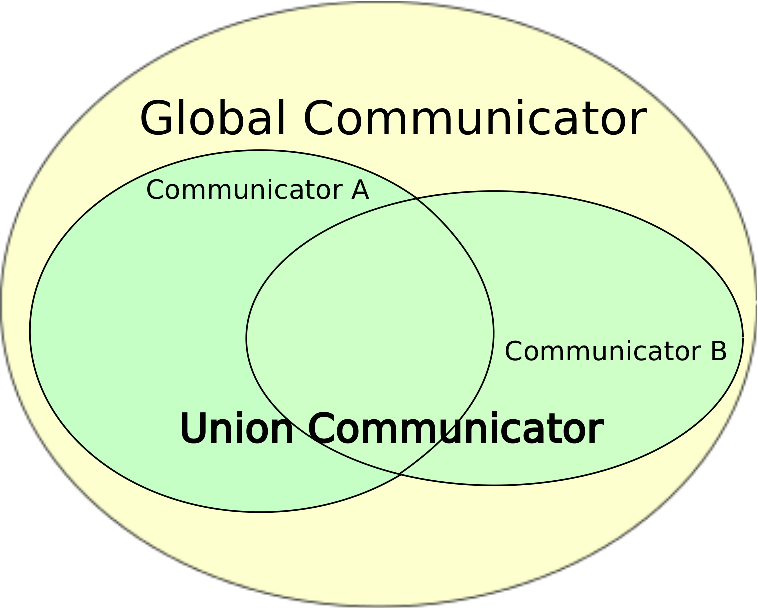
\includegraphics[width=1.7in]{union_comm.pdf}
      \end{figure}

      \begin{figure}[htpb!]
        \centering 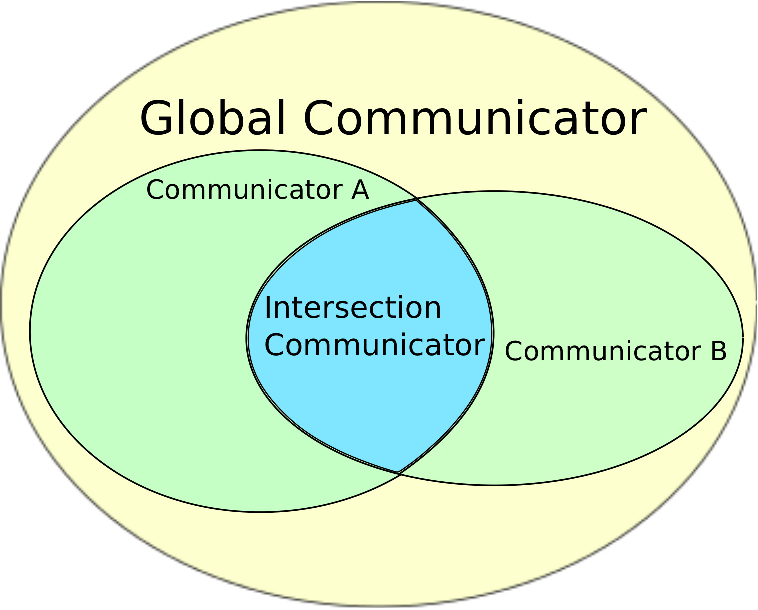
\includegraphics[width=1.7in]{intersection_comm.pdf}
      \end{figure}
    \end{column}

  \end{columns}

\end{frame}

%%---------------------------------------------------------------------------%%
\begin{frame}{Shared Domain Problems}

  \begin{columns}
    
    \begin{column}{0.5\textwidth}
      \begin{figure}[htpb!]
        \centering 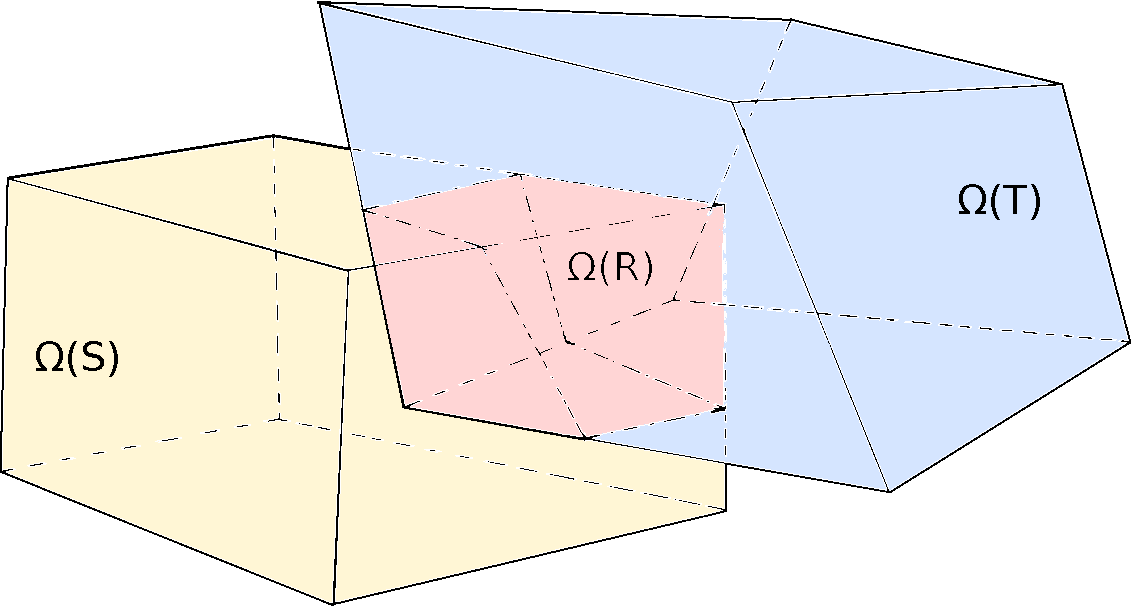
\includegraphics[width=2.5in]{overlapping_domain.pdf}
        \caption{\bf \sl Shared domain example.} {\sl $\Omega(S)$ (yellow)
          is the source geometry, $\Omega(T)$ (blue) is the target geometry,
          and $\Omega(R)$ (red) is the shared domain.}
        \label{fig:shared_domain}
      \end{figure}
    \end{column}

    \begin{column}{0.5\textwidth}
      \begin{itemize}
      \item Defined over a communicator that encapsulates the union of
        the source and target communicators
        \medskip
      \item Source and target must be of same geometric dimension
        \medskip
      \item The rendezvous algorithm leveraged to provide parallel
        topology maps for shared domains
      \end{itemize}
    \end{column}

  \end{columns}

\end{frame}

%%---------------------------------------------------------------------------%%
\begin{frame}{Parallel Topology Maps}

  \begin{itemize}
  \item An operator, $M$, that defines the translation of a field,
    $F(s)$, from a source spatial domain, $\Omega_S$, to a field,
    $G(t$), in the target spatial domain $\Omega_T$, such that
    $G(t)\leftarrow M(F(s))$ and $M: \mathbb{R}^D \rightarrow
    \mathbb{R}^D, \forall r \in \Omega_R$, where $\Omega_R$ is the
    geometric rendezvous of the source and target.
  \end{itemize}

\end{frame}

%%---------------------------------------------------------------------------%%
\begin{frame}{The Rendezvous Algorithm}

  \begin{itemize}
    \item Initially developed by the SIERRA team in the mid-2000's for
      parallel mesh-based data transfer \footnote{S. Plimpton,
        B. Hendrickson, and J. Stewart, “A parallel rendezvous
        algorithm for interpolation between multiple grids,” Journal
        of Parallel and Distributed Computing, vol. 64, pp. 266–276,
        2004}
      \medskip
    \item Creates a parallel topology map that can be used repeatedly
      for data transfer
    \item Map execution uses asynchronous strategy (posts and waits)
      with minimal messages
    \item Effectively $N*log(N)$ time complexity for parallel topology
      map generation
      \medskip
    \item Relies on the generation of a secondary decomposition of the
      source and target meshes with a geometric based paritioning
      (RCB)
  \end{itemize}

\end{frame}

%%---------------------------------------------------------------------------%%
\begin{frame}{The Rendezvous Decomposition}

  \begin{columns}

    \begin{column}{0.33\textwidth}
      \begin{figure}[htpb!]
        \centering 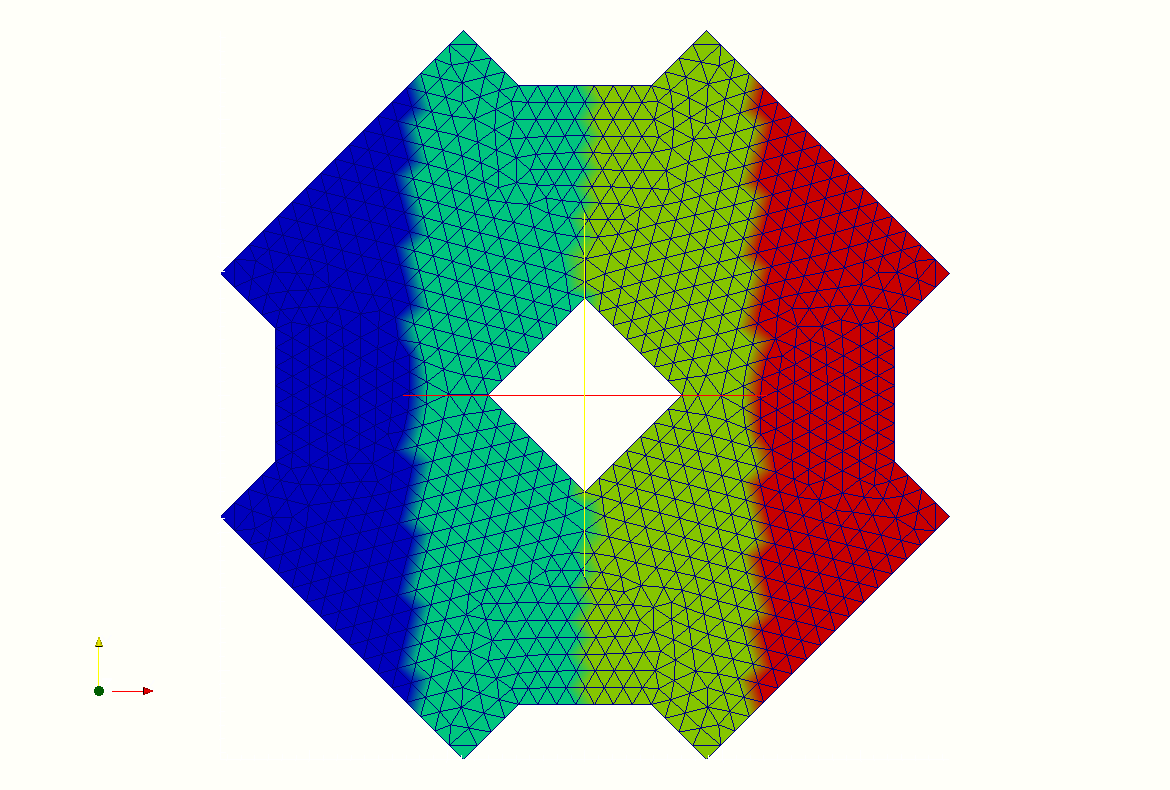
\includegraphics[width=2in]{tri_part.png}
        \caption{\small \sl Source mesh for 2D shared domain
          example.}
        \label{fig:source_mesh}
      \end{figure}
    \end{column}

    \begin{column}{0.33\textwidth}
      \begin{figure}[htpb!]
        \centering 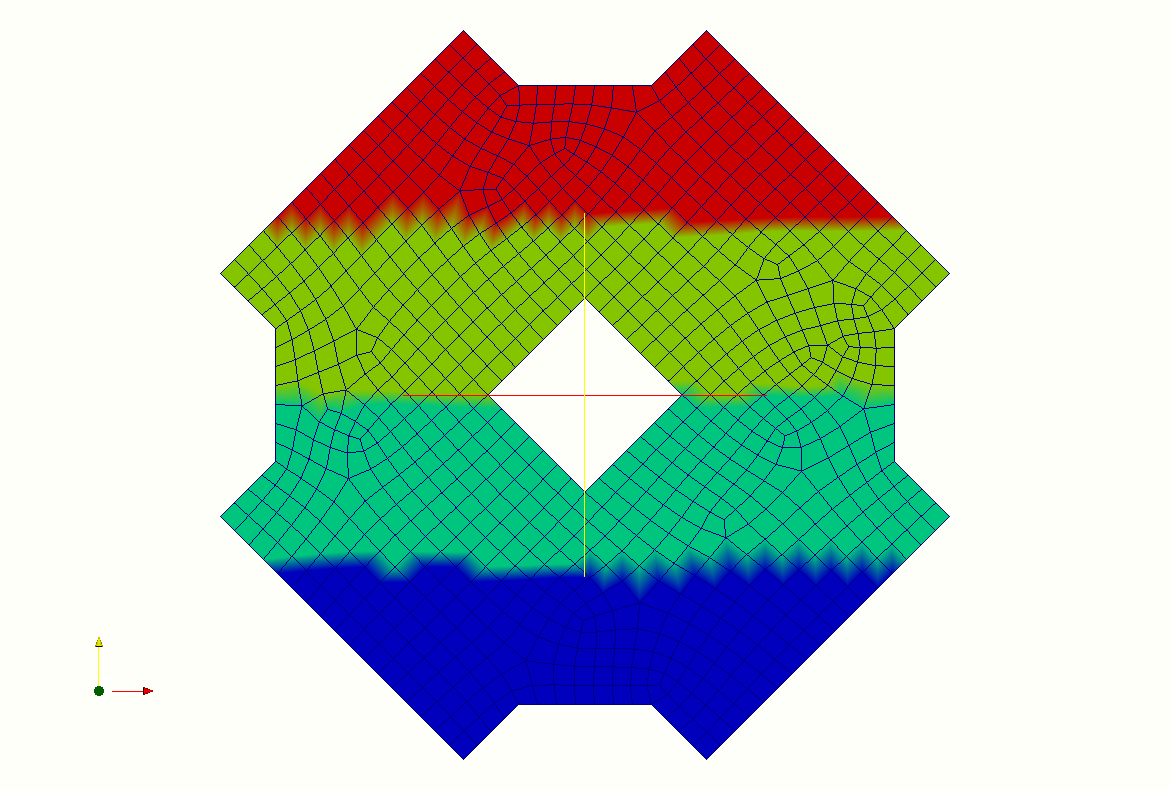
\includegraphics[width=2in]{quad_part.png}
        \caption{\small \sl Target mesh for 2D shared domain
          example.}
        \label{fig:target_mesh}
      \end{figure}
    \end{column}

    \begin{column}{0.33\textwidth}
      \begin{figure}[htpb!]
        \centering 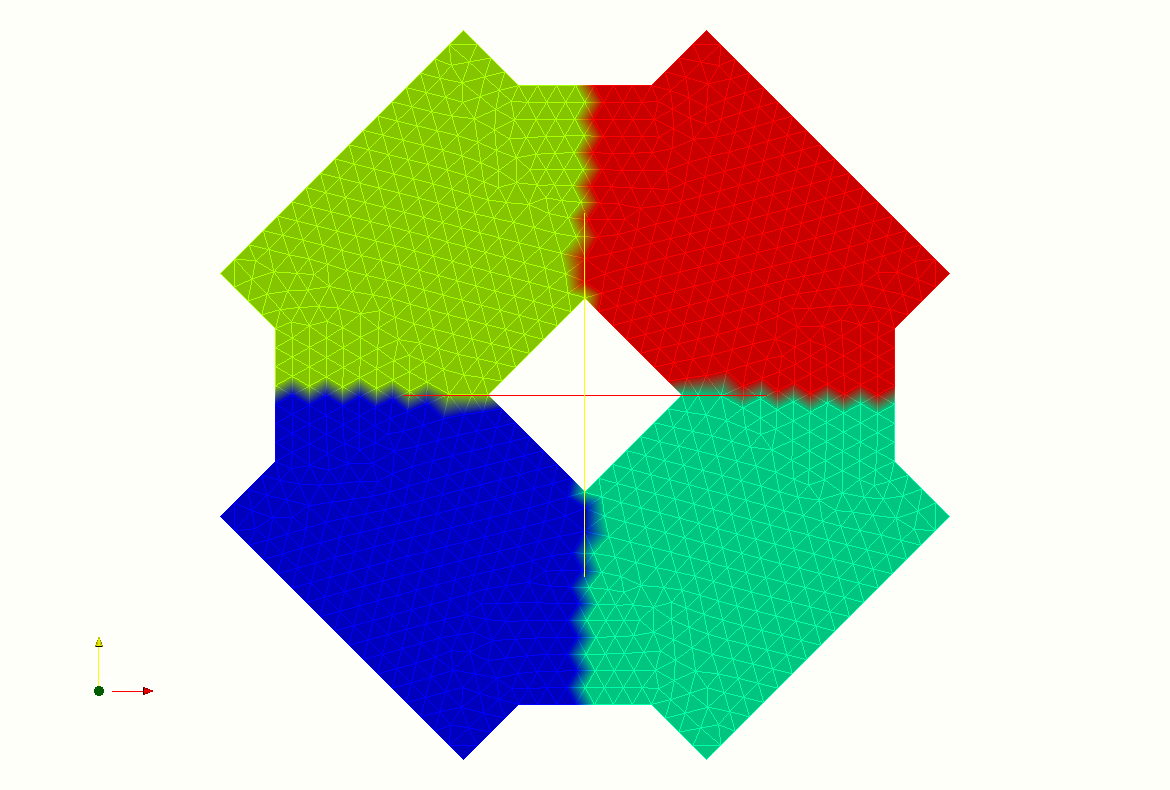
\includegraphics[width=2in]{tri_rend.png}
        \caption{\small \sl Rendezvous decomposition for 2D shared domain
          example.}
        \label{fig:rendezvous_part}
      \end{figure}
    \end{column}

  \end{columns}

\end{frame}

%%---------------------------------------------------------------------------%%
\begin{frame}{Searching the Rendezvous Decomposition}
  
  \begin{itemize}
  \item Hierarchical parallel search tree
    \medskip
  \item Rendezvous decomposition provides parallel search
    \medskip
  \item kD-tree provides on-process proximity search
    \medskip
  \item Newton iterations provide final point location
    \medskip
  \item Results in reasonable scalability
  \end{itemize}

\end{frame}

%%---------------------------------------------------------------------------%%
\begin{frame}{DTK Implementation Scaling Results}

  \begin{columns}
    
    \begin{column}{0.5\textwidth}
      \begin{itemize}
      \item Mesh-to-mesh transfer
      \item Worst case scenario study (all-to-all)
        \medskip
      \item Qualitatively similar to the SIERRA results
        \medskip
      \item Largest problems so for over 1.0E9 elements and 1.0E5 cores
      \end{itemize}
    \end{column}

    \begin{column}{0.5\textwidth}
      \centering
      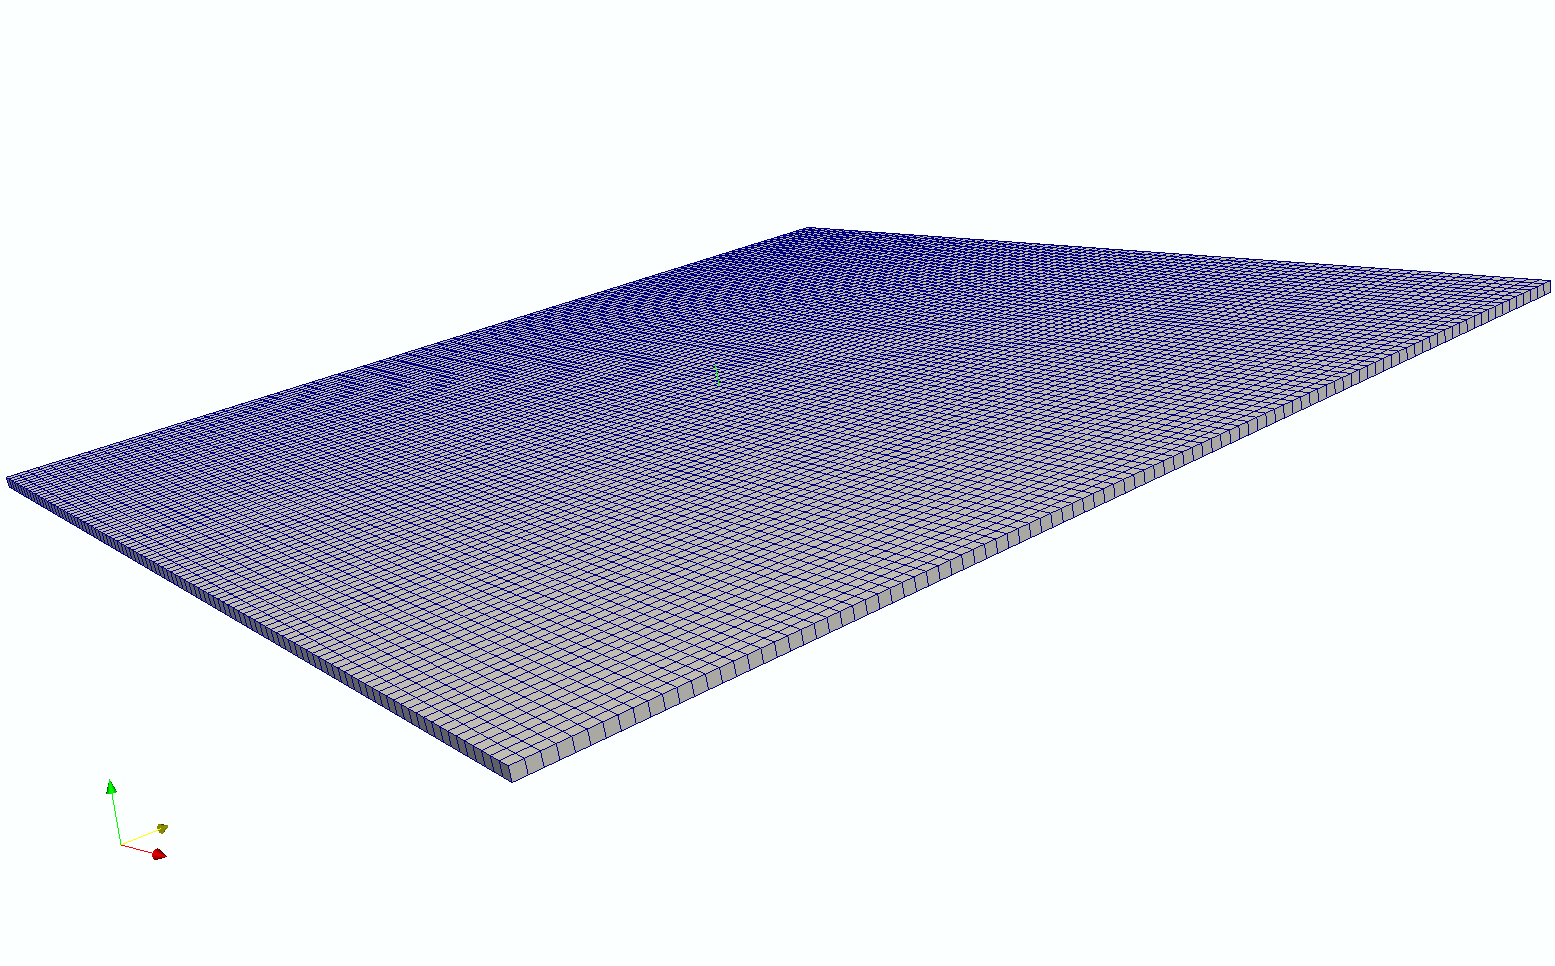
\includegraphics[width=2.4in]{mesh.png}
    \end{column}

  \end{columns}

\end{frame}

%%---------------------------------------------------------------------------%%
\begin{frame}{Strong Scaling}

  \begin{figure}[htpb!]
    \centering
    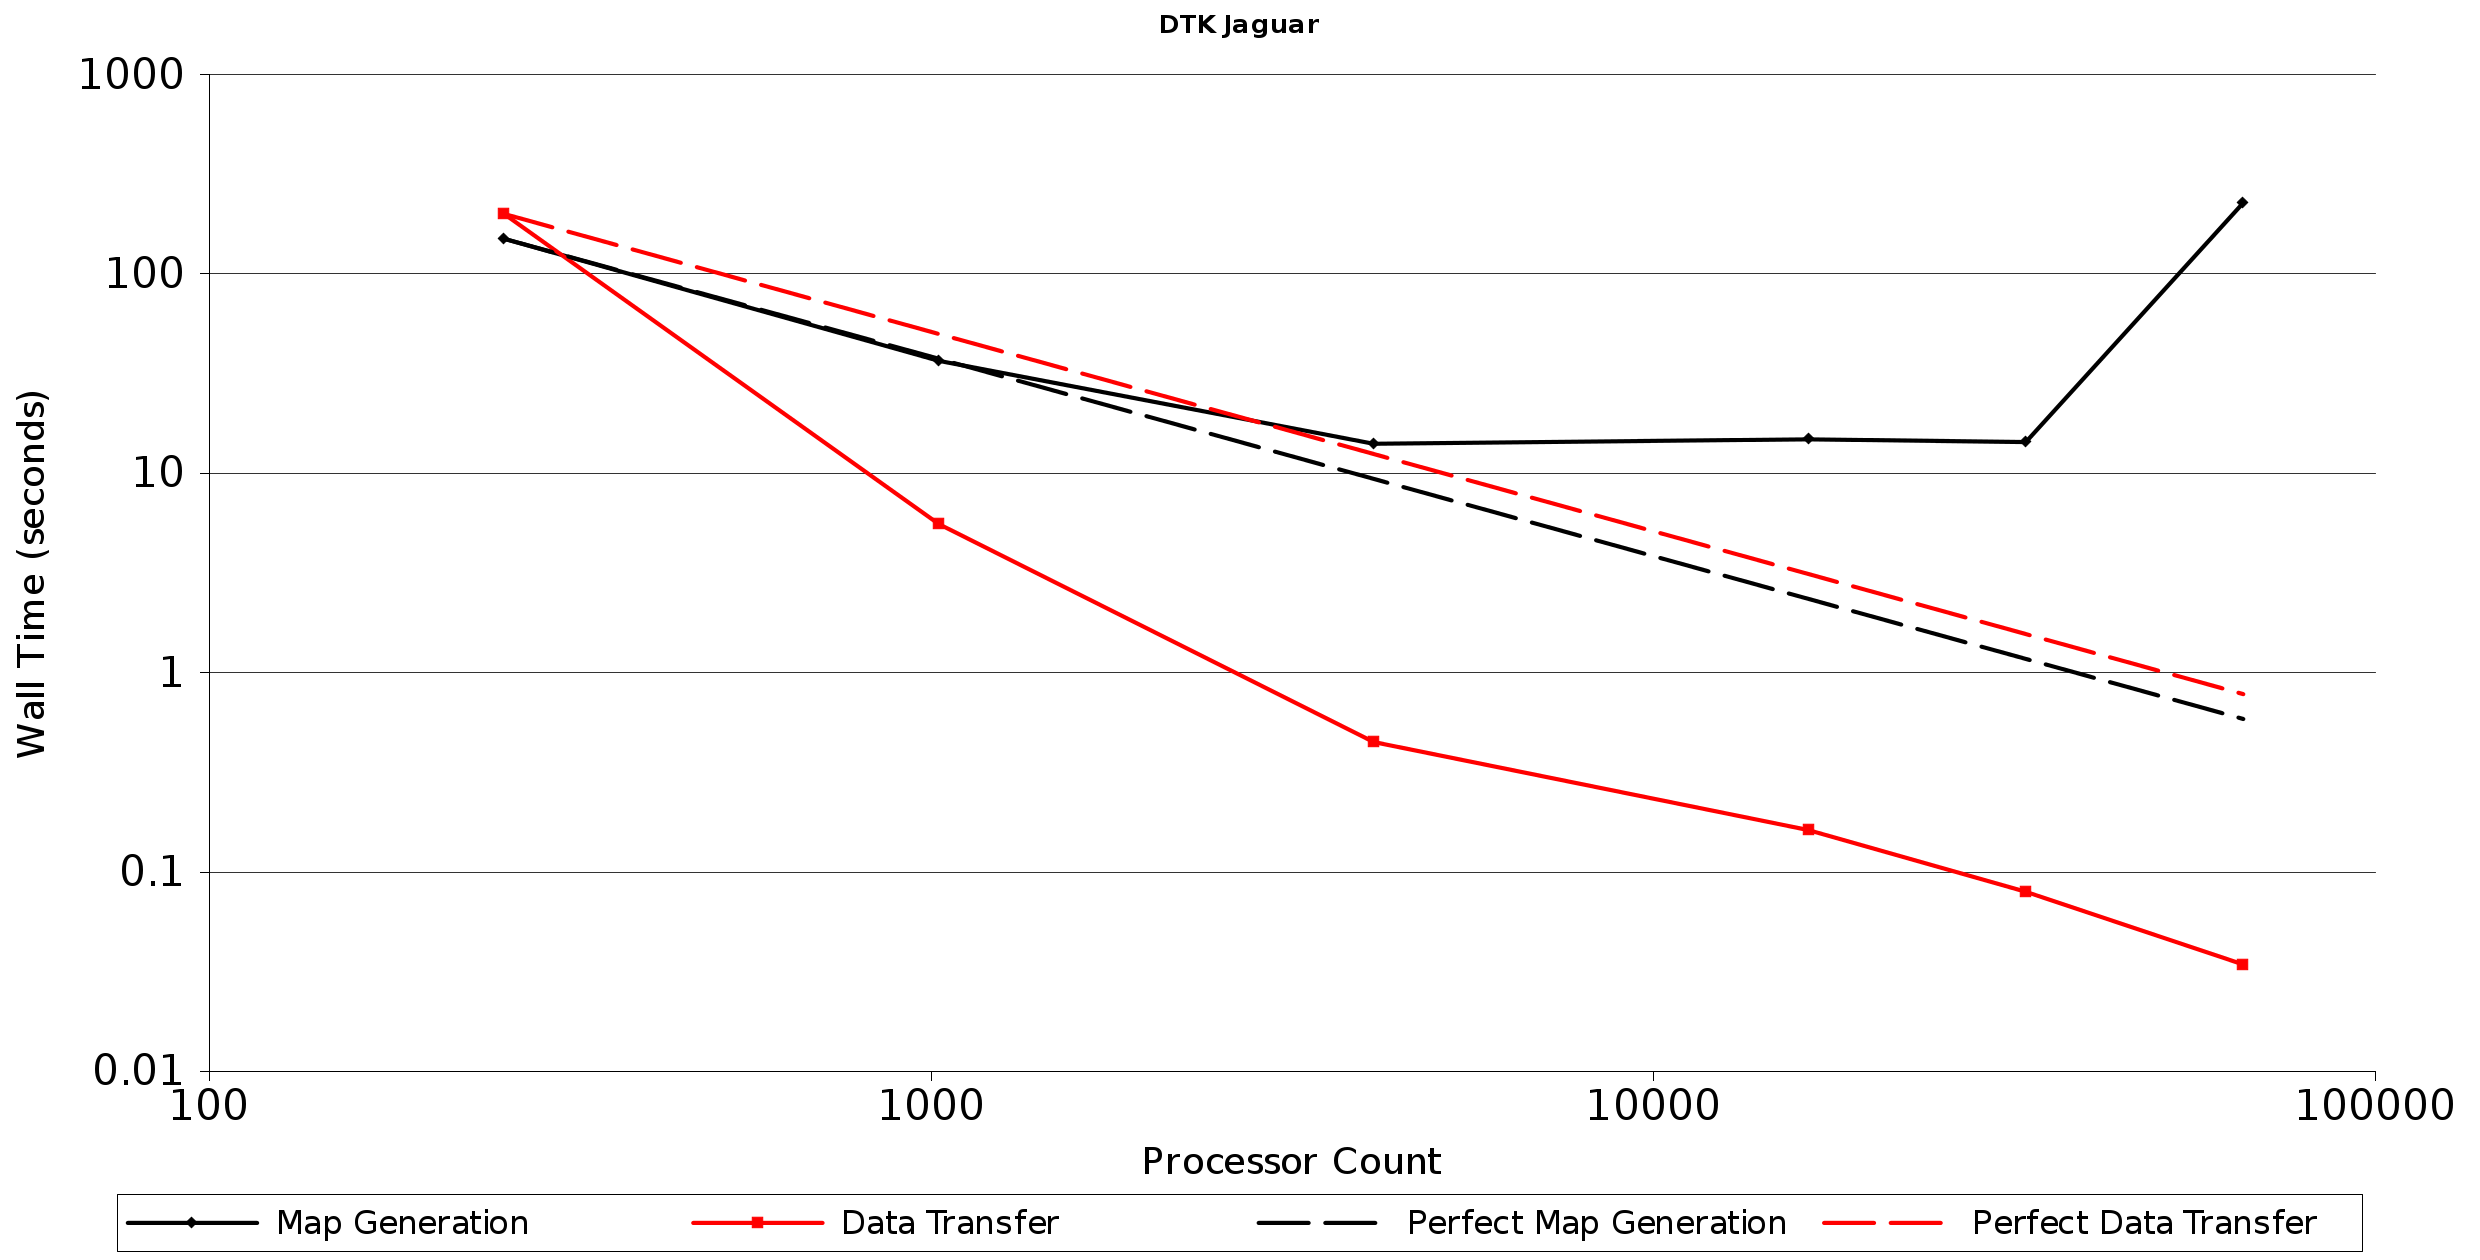
\includegraphics[width=4in]{StrongScaling.png}
    \caption{Strong scaling study results. The solid black curve reports
      the wall time to generate the mapping vs. number of processors
      while the solid red curve reports the wall time to transfer the
      data vs. number of processors. The dashed lines give
      perfect strong scaling the map generation (black) and the data
      transfer (red).}
    \label{fig:strong_scaling}
  \end{figure}

\end{frame}

%%---------------------------------------------------------------------------%%
\begin{frame}{Weak Scaling}

  \begin{figure}[ht!]
    \centering
    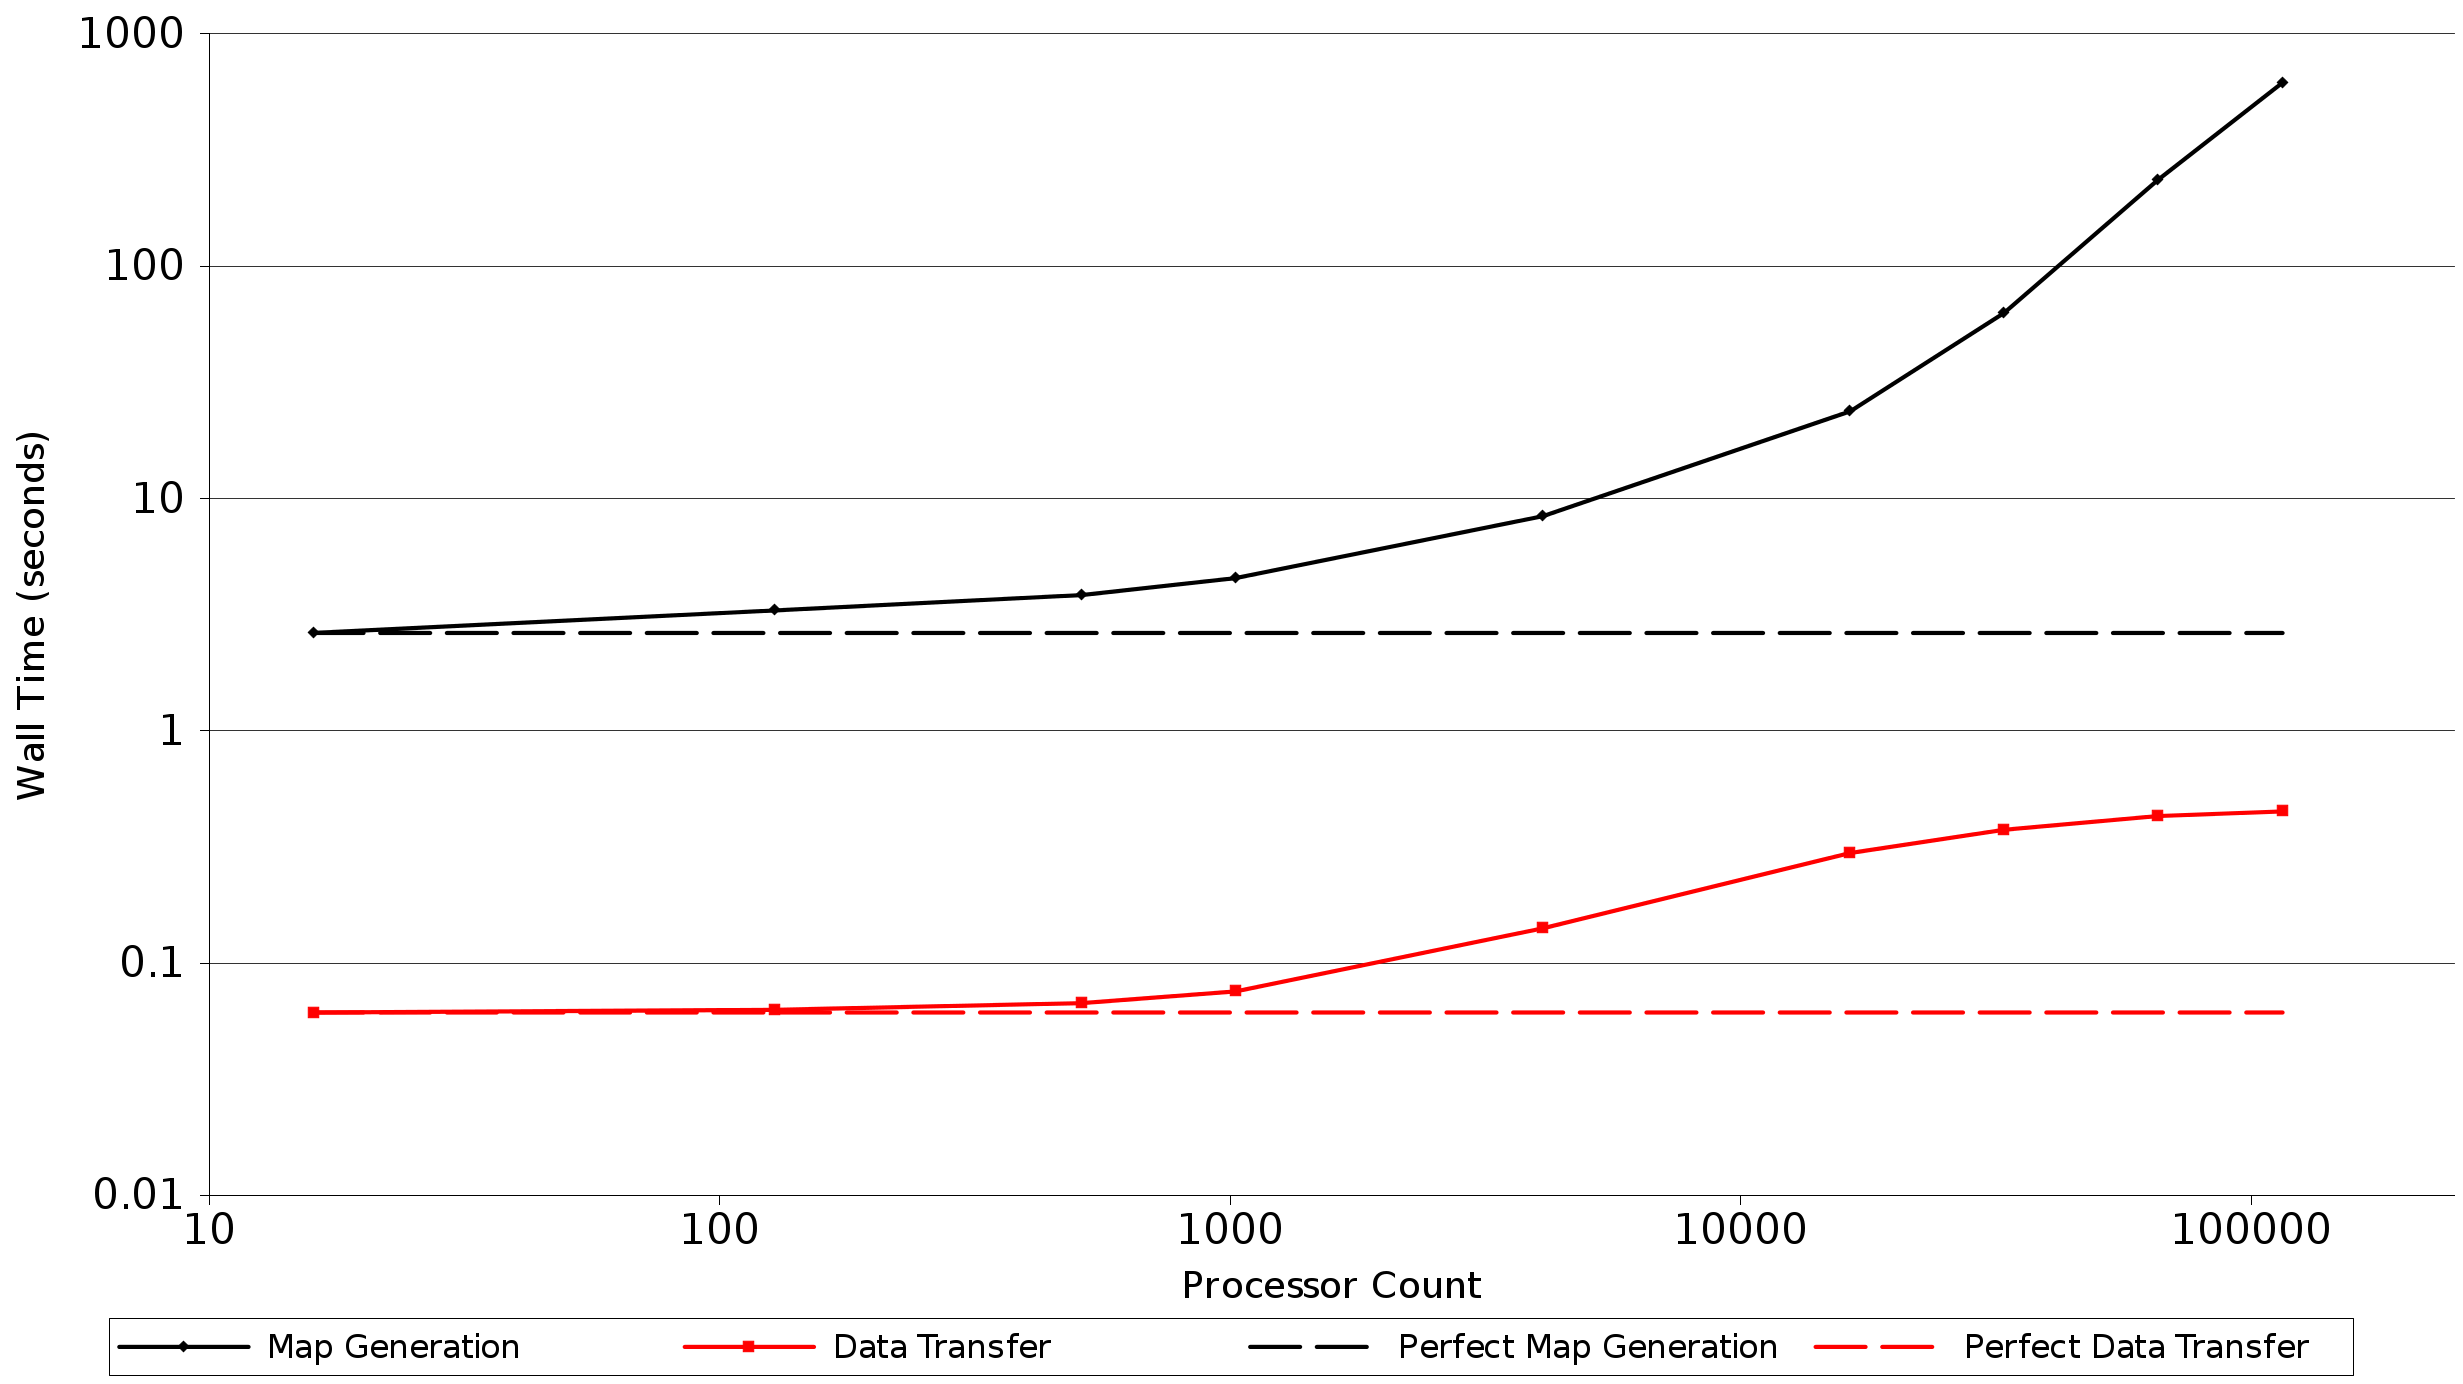
\includegraphics[width=4in]{WeakScaling.png}
    \caption{Weak scaling study results. The solid black curve reports
      the wall time to generate the mapping vs. number of processors
      while the solid red curve reports the wall time to transfer the
      data vs. number of processors. The dashed lines give
      perfect weak scaling the map generation (black) and the data
      transfer (red).}
    \label{fig:weak_scaling}
  \end{figure}

\end{frame}

%%---------------------------------------------------------------------------%%
\begin{frame}{Getting Data into DTK: The Mesh}
  
  \begin{itemize}
    \item Meshes are viewed as geometric structures
      \medskip
    \item A subset of total mesh information is needed:
      \medskip
      \begin{itemize}
        \item Vertex coordinates
        \item Element topology
        \item Element connectivity
        \item Connectivity permutation
      \end{itemize}
      \medskip
    \item Parallel information is not required
      \medskip
    \item A communicator and global IDs are required
  \end{itemize}

\end{frame}

%%---------------------------------------------------------------------------%%
\begin{frame}{Mesh Vertices and Elements}

  \begin{columns}
    
    \begin{column}{0.5\textwidth}
      \begin{figure}[htpb!]
        \centering 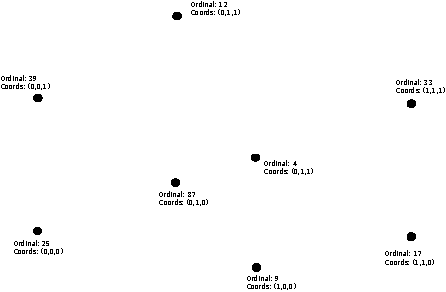
\includegraphics[width=2.25in]{hex_nodes.pdf}
        \caption{\bf \sl Basic vertex description for a mesh.}{\sl
          Each vertex is required to have a unique global ID}
      \end{figure}
    \end{column}

    \begin{column}{0.5\textwidth}
      \begin{figure}[htpb!]
        \centering 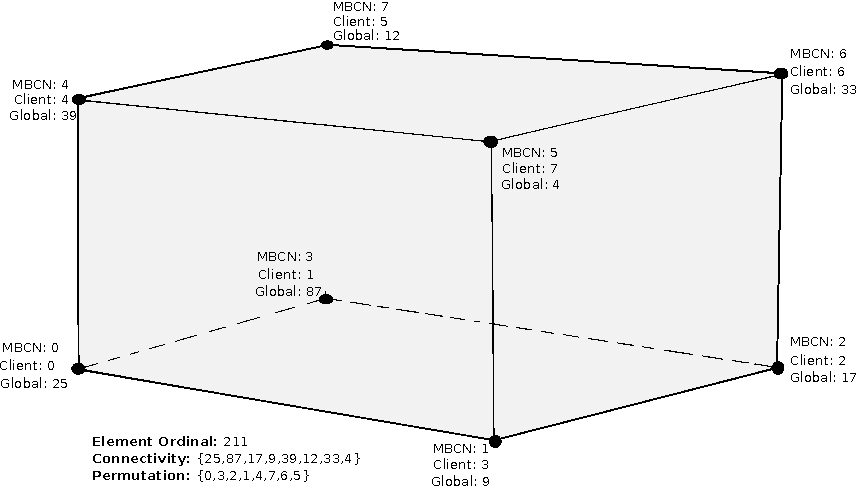
\includegraphics[width=2.25in]{hex_element.pdf}
        \caption{\bf \sl Basic element description for a mesh.}{\sl
          Each element is required to have a unique global ID}
      \end{figure}
    \end{column}

  \end{columns}

\end{frame}

%%---------------------------------------------------------------------------%%
\begin{frame}{Connectivity Permutation}

  \begin{columns}
    
    \begin{column}{0.5\textwidth}
      \begin{figure}[htpb!]
        \centering
        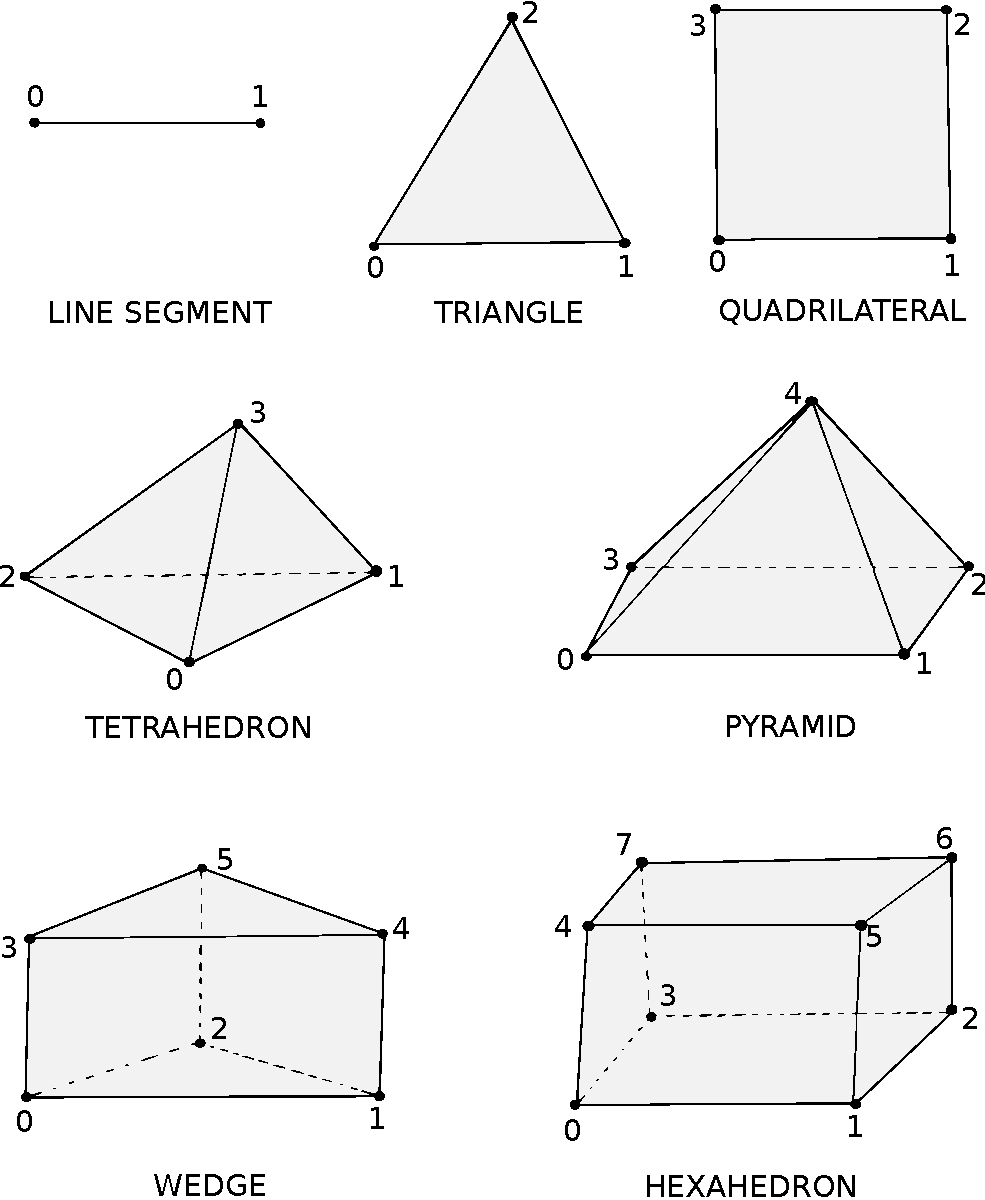
\includegraphics[width=2.5in]{Linear_Elements.pdf}
        \caption{\bf \sl Canonical vertex connectivity schemes for elements
          in DTK.}
        \label{fig:linear_elements}
      \end{figure}
    \end{column}

    \begin{column}{0.5\textwidth}
      \begin{itemize}
        \item Allow for user specification of canonical ordering
          \medskip
        \item Permutation list specifies the variation in ordering for
          a specified topology
          \medskip
        \item Support for other mesh topologies currently not offered
      \end{itemize}
    \end{column}

  \end{columns}


\end{frame}

%%---------------------------------------------------------------------------%%
\begin{frame}{Meshes of Multiple Topologies}

  \begin{itemize}
  \item All topologies in a mesh must be of the same dimension
  \item Each topology contained in a block
  \item Can have multiple blocks of the same topology
  \end{itemize}


  \begin{figure}[htpb!]
    \centering 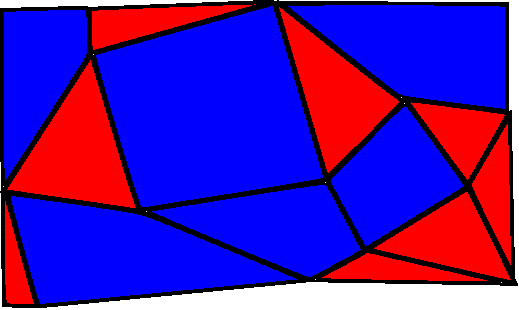
\includegraphics[width=2.5in]{hybrid_mesh.pdf}
    \caption{\bf \sl Hybrid mesh example.} {\sl Quadrilaterals (blue)
      must be specified in a different mesh block than the triangles
      (red). Both blocks can contain the mutual mesh vertices that
      construct their elements.}
    \label{fig:hybrid_mesh}
  \end{figure}

\end{frame}

%%---------------------------------------------------------------------------%%

\end{document}
